%!TEX root = ../thesis.tex

\chapter{绪论}

\section{研究背景及意义}

大气污染物的环境和气候效应不仅取决于其浓度的多少,在很大程度上还决定于其在大气中的垂直分布。而深对流是将边界层空气及气溶胶传输到对流层上层和平流层下层(UTLS)的重要机制\citep{Chatfield.1984,Dickerson.1987,Pickering.1989,Yin.2002}。
在深对流系统中,污染物从地面传输到对流层上层只需要几分钟至一个小时\citep{Skamarock.2000}。
研究学者通过结合外场观测\citep{Dickerson.1987,Pickering.1996,Bertram.2007,Apel.2012,Pan.2017}
和卫星资料\citep{Halland.2009,Barth.2012,Livesey.2013,Jensen.2015}
现已证明深对流输送会影响UTLS的水汽和化学成分。

根据对全球对流层大气组分的收支情况的估计,\citet{Cotton.1995}指出每年大约有90次
由对流造成的边界层大气的垂直输送,其中很大一部分能够到达对流层的上层。
在低纬度地区,对流每天以约8\%的速率向对流层上层输送,
这与由光化学过程控制的氢氧化物[HO$_x$ = 羟基(OH)+ 过氧化氢自由基(HO$_2$)]
和氮氧化物[NO$_x$ = 一氧化氮(NO)+ 二氧化氮(NO$_2$)]的产生率相当,
深对流甚至可以直接将边界层大气输送至UTLS\citep{Prather.1997},
其中臭氧(O$_3$)前体物的垂直传输显著提高了对流层上层云砧出流区中O$_3$的产量\citep{Pickering.1990,Pickering.1992,Pickering.1992a}。
由于在对流层上层风速较大,污染气体的生命期或滞留时间也更长,所以前体物的影响范围更广。
就气候辐射强迫而言,对流层O$_3$是第三大重要的温室气体\citep{Myhre.2013},仅次于二氧化碳(CO$_2$)和甲烷(CH$_4$)。

与此同时,通过深对流云顶过冲(overshooting)侵入平流层的湿空气,会增加平流层下层水汽\citep{Homeyer.2014},
这是平流层下层水汽变化的主要原因之一。
而平流层水汽是年代纪全球气候变化的关键驱动力\citep{Solomon.2010}。 此外,深对流传输也会影响气溶胶垂直分布,这是气溶胶辐射强迫的重要组成部分\citep{Mishra.2012,Park.2015}。
综上所述,对流输送可改变高层污染气体和气溶胶在区域和全球大气中的循环\citep{Clarisse.2011},并通过云和降水过程改变边界层气溶胶浓度来调节全球气候\citep{Taylor.1997}。

除此之外,深对流云中的闪电现象也会对大气污染物的垂直分布产生影响。
如Zel'dovich机理所述\citep{Zeldovich.1967},
闪电在高温下通过分解氧分子(O$_2$)和氮分子(N$_2$)产生NO,接着NO迅速氧化为NO$_2$并达到平衡。
自从\citet{Liebig.1827}提出闪电固氮的机制以来,闪电一直被认为是NO$_x$的一个主要来源\citep{Hutchinson.1954}。
闪电NO$_x$(LNO$_x$)的全球产量大约为2–8 Tg氮每年,是对流层上层NO$_x$的主要来源\citep{Galloway.2004,Schumann.2007}。
新的化学机制表明,NO$_x$在对流层上层的寿命取决于与雷暴的距离,在雷暴附近该寿命为$\sim$3小时,而远离雷暴处可达0.5--1.5天\citep{Nault.2016,Nault.2017},从而导致对流云出流区的O$_3$浓度增高\citep{Pickering.1996,Hauglustaine.2001,DeCaria.2005}。
因为O$_3$是强氧化剂和紫外线吸收剂\citep{Myhre.2013},所以LNO$_x$对O$_3$的贡献也会影响气候强迫。
此外,电晕放电亦可直接产生O$_3$\citep{Minschwaner.2008,Kotsakis.2017}。

因此,了解大气污染物在深对流云中的传输和清除过程以及LNO$_x$的产量,
对于理解大气污染物的远距离输送、与云和辐射的相互作用,以及对空气质量和气候变化的影响具有重要意义。



\section{国内外研究进展}

\subsection{深对流中闪电氮氧化物的观测和估算} \label{sec:intro_lnox}

深对流伴随的闪电对大气痕量气体(O$_3$、NO、NO$_2$等)有着重大影响\citep{DeCaria.2005,Schumann.2007,Ott.2010,Banerjee.2014}。
\citet{Levy.1996}指出,对流层上层的NO$_x$主要由闪电活动产生,生命史较长,控制着对流层O$_3$和OH自由基的含量,进而会给大气层乃至全球气候带来至关重要的影响。在热带和亚热带地区,对流层顶70\%以上的NO$_x$来自闪电,在一些高纬度地区的夏季,这一比例也可达20\%以上\citep{Jourdain.2001,Martin.2002}。
此外,前人也开展了闪电对O$_3$垂直分布影响的研究。
在大陆边界层内排放的O$_3$前体物,可通过上升气流进入自由对流层,和LNO$_x$一起参与生成O$_3$的光化学反应\citep{Bond.2002}。
\citet{Tie.2001}利用全球化学传输模式(MOZART)发现闪电可导致NO$_x$、HNO$_3$和过氧乙酰硝酸酯(PAN)显著增加。
\citet{Cooper.2009}指出闪电对美国东部地区对流层上层NO$_x$的贡献高于80\%,
而夏季对流层上层的反气旋可将LNO$_x$与由对流输送的O$_3$及其前体物聚在一起,产生北美东部夏季对流层上层O$_3$的高值区。
\citet{Kang.2020}将美国国家闪电探测网(NDLN)资料融合进社区多尺度空气质量模式系统(CMAQ)的闪电模块,发现美国山区LNO$_x$与人为排放NO$_x$相当,每日8小时最大O$_3$值因此提高17 ppbv,且更接近地表观测值。

局地或全球LNO$_x$产量主要通过野外观测及实验室试验结果推算得到。
早期主要是结合一些地面观测仪器来分析雷暴下部或地闪附近的NO$_x$含量。
从上世纪90 年代开始,欧美对LNO$_x$的空中观测试验越来越多,如LINOX试验\citep{Huntrieser.1998}、 MOZAIC试验\citep{Marenco.1998}、
STERAO试验\citep{Dye.2000}、EULINOX试验\citep{Holler.2000}、TROCCINOX试验\citep{Huntrieser.2007}等。
这些试验利用配备了测量NO$_x$、O$_3$、CO$_2$等痕量气体设备的飞机进行穿云观测,可直接得到雷暴云中及附近地区NO$_x$的变化。
表\ref{table:NO/NOx}详细列出了2005年之前在雷暴附近开展野外观测的研究结果。

{
\centering
\scriptsize
\begin{longtable}
{|p{3em}|p{5.2em}|p{3.1em}|p{1.6em}|p{3em}|p{4em}|p{3.5em}|p{4em}|p{4em}|p{8em}|}
\caption{试验个例\\
Table \ref{table:NO/NOx}. Experiments.}
\label{table:NO/NOx} \\
\hline
年份 & 试验,地区  & 仪器$^a$  & 物种 & 平均值 (nmol mol$^{−1}$) &
平均尺度 (km) $^b$  &  峰值 \newline(nmol mol$^{−1}$)  &  峰值 \newline 持续时间  & 峰值高度(km) &   参考文献 \\ \hline
$\sim$1960s & 德国南部万克山观测站              & KI     & NO$_2$ & -   &  -    &  $\sim$3, <50  & -    & 1.7   &  \citet{Reiter.1970} \\ \hline
1981年四月   & 伊利诺伊州,阿尔贡市              & CL     & NO$_x$ & -   &  -    &  20            & 40 s  & 地表  &  \citet{Drapcho.1983} \\ \hline
1982年十二月 & 法兰克福–圣保罗航班               & CL     & NO$_x$ & 0.3 & > 100 &  0.5           & ~ min &  9.5 & \citet{Dickerson.1984} \\ \hline
1983年十一月 & GTE / CITE 1A,夏威夷附近的太平洋 & TP-LIF & NO  & 1    & 40    &   1            & 2 min & 9    & \citet{Chameides.1987,Davis.1987} \\ \hline
1983年      & 美国中西部                       & CL     & NO$_x$ & 0.6 & -     & 1.2            & 10 s  & 10–-11 & \citet{Dickerson.1987} \\ \hline
1985年六月   & PRE-STORM,科罗拉多州大平原       & CL     & NO  & 0.3 & -     & 1.2,4.1       & 20--60 s, 10 s &  10.6  &  \citet{Luke.1992} \\ \hline
1985年七月十二日  & GTE / ABLE 2A,巴西马瑙斯附近的亚马逊地区 & CL  & NO  & 0.06 & 60-100 & 0.17  & 5-40 s & 5  & \citet{Torres.1988} \\ \hline
1989年六月   & NDTP,北达科他州                 & CL     & NO  & 0.25  & -   & 0.9            & 20 s   &  11  & \citet{Poulida.1996} \\ \hline
1989年七--八月 &  ELCHEM,新墨西哥州            & CL      & NO  & 0.1--0.8 & 20--44  & 1.3--1.9 & 4 s  & 10.5--10.9   & \citet{Ridley.1996} \\ \hline
1992年九月27日  & GTE / TRACE A,巴西塞拉多,6$^{\circ}$--12$^{\circ}$S & TP-LIF & NO$_x$ & 0.3--0.9 & - &  1.4 & 3 min  & 9.5 & \citet{Pickering.1996} \\ \hline
1994年二月    & PEM-West,西太平洋,4$^{\circ}$--10$^{\circ}$S & CL  &  NO  & 0.05--0.2 &~100 & 0.2 & 30 s  &  9.5 & \citet{Kawakami.1997} \\ \hline
1995年七月一日 &  POLINAT,爱尔兰               & CL      & NO  & 0.6  & 27--90 & - &  -  & 9.5 & \citet{Huntrieser.1996} \\ \hline
1996年六-七月  & STERAO,科罗拉多州             & CL      & NO  & 0.2--0.8 & 20--40  & 4.2, 19 & 1-10 s,(100-960 m) & 7-12 s &  \citet{Dye.2000} \\ \hline
1996年七月    & LINOX,德国南部                & CL       & NO NO$_x$ & 0.4--1.3,0.8--2.2 & 10--45  & 3.8,20 & 2 s & 8.2, 9 & \citet{Huntrieser.1998} \\ \hline
1997年八月和十一月 & NO$_x$AR / POLINAT-2,北大西洋  & CL     & NO  & 0.8, 3  & 1000, 300 & -   & -  & - & \citet{Jeker.2000} \\ \hline
1998年七月 & EULINOX,德国南部                  & CL      & NO$_x$  & 0.5--3.0 & 15--60 &  25, >20 &  2--10 s & 8--10 &    \citet{Huntrieser.2002} \\ \hline
1998年七月 & STREAM,加拿大安大略省                &  CL     & NO  & 0.6--2    & 100  & 2.5 & 1 min &  10 & \citet{Lange.2001} \\ \hline
1999年九月 & BIBLE,达尔文和比亚克之间的太平洋     & CL      & NO  & 0.1--0.3 & 800   & 1.4 & 1 s & 13  & \citet{Kondo.2003} \\ \hline
2000年三月 & INCA,南美西海岸                    & CL     & NO  & 0.04--0.8  & 400 & 1.3 & 1 s & 11.5 & \citet{Baehr.2003} \\ \hline
2000年十二月九日 & BIBLE-C,靠近澳大利亚达尔文     & CL     & NO$_x$  & 0.4       & 140-620 & 1.6 & 10 s  &  11.5--14 & \citet{Koike.2007} \\ \hline
2002年七月 & CRYSTAL FACE,佛罗里达             & CL      & NO  & 1--4      & 60--120 & 9.5, 325 & 0.3 s & 13.8 & \citet{Ridley.2005} \\ \hline
2004年一月至三月,2005年二月 & TROCCINOX 巴西,圣保罗州 & CL & NO  & 0.5--1.5 & 25--40  & 45  & 1 s & 8 &  \citet{Huntrieser.2007} \\ \hline
\end{longtable}
\begin{tablenotes}
\linespread{1}\footnotesize
\item $^a$ CL:来自NO + O$_3$反应的化学发光分析; KI:基于NO$_2$气体与稀释的KI溶液之间的化学反应; TP-LIF:双光子激光诱导的荧光。
\item $^b$ 平均NO或NO$_x$增强的水平平均尺度; -: 无资料。
\item 来源:\citet{Schumann.2007}
\end{tablenotes}
}

闪电外推法将全球LNO$_x$的产率定义为:每次闪电LNO$_x$的产率与全球闪电频率的乘积\citep{Lawrence.1995}。
一次闪电的LNO$_x$产率可由单次放电单位能量[或峰值电流,\citet{Wang.1998}]乘以一次闪电的放电能量(或峰值电流)来确定。
此外,还有一种方法是将单位闪电长度的LNO$_x$产率与闪电长度的估算值相乘。
其他方法则是直接估算单次闪电的LNO$_x$产率。
所有这些方法都基于一个假设,一组估算值代表全球的闪电特性。
表\ref{table:LNOx/J}列出了该方法估算所得的LNO$_x$产率,该值的范围是1--50$\times$10$^{16}$分子J$^{-1}$。
如果消耗所有放电能量都用来分裂分子氮的三键(0.94 MJ mol$^{-1}$),
则LNO$_x$产量最多可达到64$\times$10$^{16}$分子J$^{-1}$。
\citet{Wang.1998}指出,LNO$_x$并不是闪电放电中能量转化为热量的单一函数,而是随大气压(近似线性)和峰值电流(近似二次方)增加。
例如,地表的峰值电流从10 kA增加到30 kA,NO分子的产率从15$\times$10$^{16}$ J$^{-1}$增加到40$\times$10$^{16}$ J$^{-1}$。
NO生成量与闪电峰值电流和环境气压之间的相关性,为估算LNO$_x$提供了一种新的方法,
即通过识别闪电和峰值电流的雷电探测系统来估算每次闪电的LNO$_x$产量。
然而可惜的是,像OTD这样的卫星系统虽然可以在全球范围内识别与闪电能量相关的辐射\citep{Baker.1999},但不能识别闪电的峰值电流。


一些飞机试验通过测量雷暴附近闪电烟羽中NO$_x$的浓度,得出单位闪电长度的LNO$_x$产量(表\ref{table:LNOx/length})。
为了将这些值外推至每次闪电的LNO$_x$产量,我们需要知道闪电的长度。
一些研究者使用一些典型的长度范围,如中纬度地闪(CG)长度为5--7 km,云闪(IC)长度范围为1--6 km \citep{Price.1997b},
但是详细的研究表明,闪电的长度可能更长\citep{Defer.2001,Thery.2001,Peterson.2020b}。
对于STERAO个例,从甚高频(VHF)雷电观测和模拟研究得出的闪电长度约为20--30 km\citep{Defer.2001}。
对于EULINOX超级单体,从VHF闪电和雷达观测得出的IC和CG闪电的典型长度为,IC:43 km,CG-:26.5 km,CG+:29.5 km \citep{Dotzek.2000}。
而最近的地球静止闪电测绘仪(GLM)探测到709 km长度的闪电,为WMO新的闪电长度记录\citep{Peterson.2020b}。



{
\centering
\footnotesize
\begin{longtable}
{|p{8em}|p{18em}|p{12em}|}
\caption{雷暴附近NO和NO$_x$混合比\\
Table \ref{table:LNOx/J}. The ratio of NO to NO$_x$ near storms.}
\label{table:LNOx/J} \\
\hline
LNO$_x$产量(10$^{16}$分子J$^{-1}$)   & 方法                          & 参考文献 \\ \hline
1.4 $\pm$ 0.7                                  & 实验室模拟电晕放电              & \citet{Hill.1988} \\ \hline
8.5 $\pm$ 4.7                                  & 综述                          & \citet{Lawrence.1995} \\ \hline
9 (5--17)                                    & 综述                          & \citet{Biazar.1995} \\ \hline
9 $\pm$ 2                                      & 实验室放电研究, NO/NO$_x$ 测量     & \citet{Stark.1996} \\ \hline
10                                           & 理论研究                      & \citet{Price.1997a,Price.1997b} \\ \hline
10--50                                       & 实验室试验                    & \citet{Wang.1998} \\ \hline
1.1 $\pm$ 0.2                                  & 低能火花的实验室实验            & \citet{Cook.2000} \\ \hline
15 $\pm$ 5    & 脉冲Nd-YAG激光在实验室模拟的热等离子体中产生闪电,初始温度接近10$^5$ K    & \citet{Navarro-Gonzalez.2001} \\ \hline
20--30      & 实验室同轴圆柱池中的流光放电                                       & \citet{Cooray.2005} \\ \hline
\end{longtable}\par
}


{
\centering
\footnotesize
\begin{longtable}
{|p{15em}|p{13em}|p{10em}|}
\caption{单位闪电长度的LNO$_x$产率}
\label{table:LNOx/length} \\
\hline
单位闪电长度LNO$_x$产率(10$^{21}$分子m$^{-1}$)   & 方法                          & 参考文献 \\ \hline
1.4--5.2                                     & 实验室NO测量和闪光化学模式,包括闪光长度的曲折系数3.6   & \citet{Wang.1998} \\ \hline
13                                           & 机载NO测量,二维云模式,闪电定位和跟踪系统  & \citet{Holler.1999} \\ \hline
2.5 (0.2--10)                                & 机载NO测量                     & \citet{Stith.1999} \\ \hline
2.7 (0.07--10)                               & 机载NO测量                     & \citet{Huntrieser.2002} \\ \hline
1                                            & 机载NO测量,三维云模式           & \citet{Skamarock.2003} \\ \hline
7.5                                          & 机载NO测量,三维云模式           & \citet{Ott.2007} \\ \hline
\end{longtable}\par
}


大气中每次闪电的LNO$_x$产率可通过地面观测\citep{Noxon.1976},
飞机试验\citep{Chameides.1987}和卫星探测\citep{Beirle.2004}得出。
这些方法通常区分CG和IC,因为他们有着不同的性质.

% \begin{equation}
% G = P_{\ch{CG}}f_{\ch{CG}} + P_{\ch{IC}}f_{\ch{IC}}
% \end{equation}

% \begin{equation}
% f_f  = f_{\ch{CG}}  + f_{\ch{IC}}
% \end{equation}


% 闪电外推法对产率比值$Z$ = $P_{\ch{IC}}$ / P_{\ch{CG}},即单次CG和IC闪电形成的NO$_x$分子数的比值,非常敏感\citep{Bond.2002}。
% 若采取云地闪比例(f_{\ch{IC}} / f_{\ch{CG}})为3,Z = 1时的总产率G是Z = 0.1时的3倍\citep{Gallardo.1996,Ridley.2004,Ridley.2005}。
闪电外推法对产率比值非常敏感\citep{Bond.2002},然而云地闪比例和云地闪产率之比都有很大不确定性。
云地闪比例在雷暴生命周期中变化很大,并且有观测显示该比例可超过100 \citep{Dye.2000,DeCaria.2005,Ott.2007}。
一些理论研究\citep{Cooray.1997}和实验室结果\citep{Cooray.2005}得出云地闪产率为1。
除此以外,将云模式模拟、闪电观测以及机载测量应用于STERAO \citep{DeCaria.2000}、EULINOX \citep{Fehr.2004}和CRYSTAL-FACE试验的结果表示,IC产生的NO量与CG相同。
图\ref{figure:lnox_production_Schumann}总结了部分理论、实验室研究、野外观测和综述研究得出的单次闪电LNO$_x$的产量。
由此可知,每次闪电低于3$\times$10$^{25}$分子的数值主要来自1980年代的理论研究和一些实验室研究。
当用如今的闪电频率和闪电能量的知识重新计算,这些早期结果中的许多数值将会产生变化,目前的产率估算与近年来越来越多的观测相一致。


\begin{figure}[H]
\centering
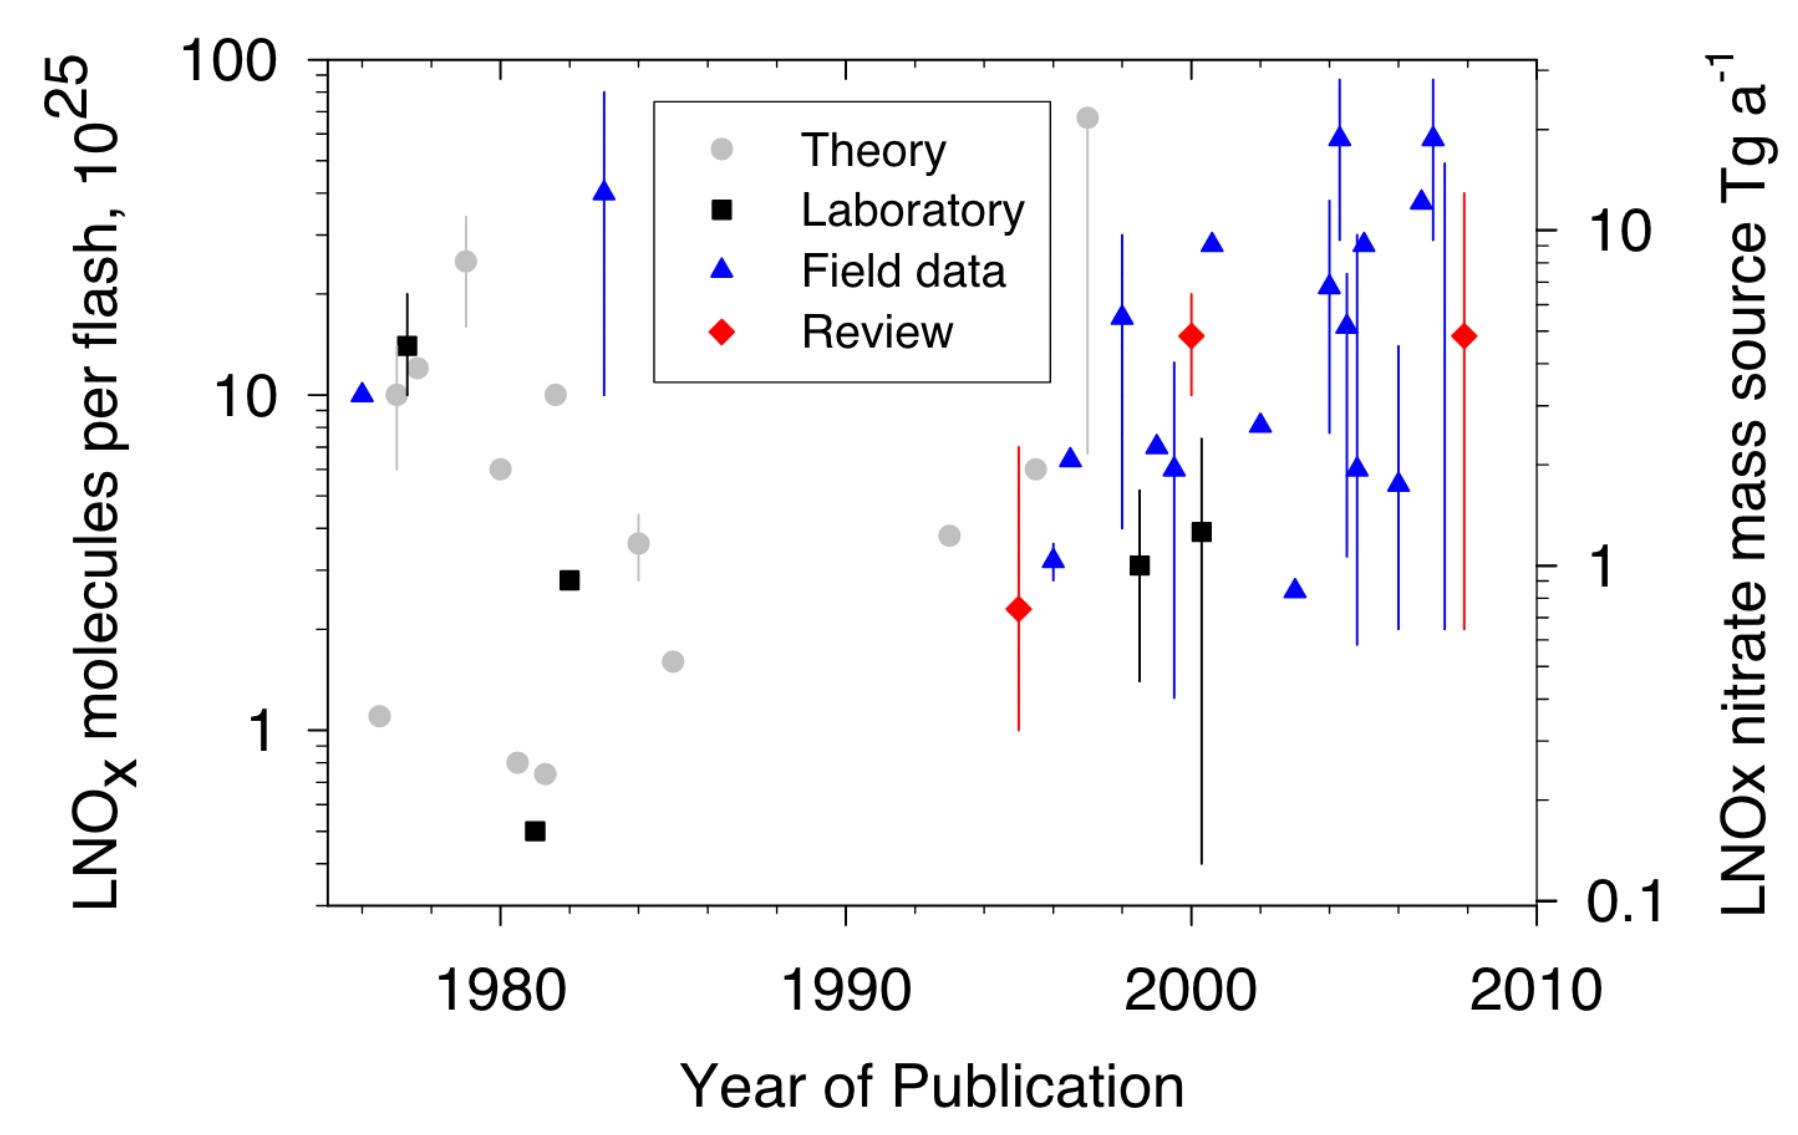
\includegraphics[width=0.8\textwidth]{./figures/lnox_production_Schumann.png}
\caption{不同年份的理论、实验室和外场观测以及综述中LNO$_x$的产率(10$^{25}$个分子)\\
Figure \ref{figure:lnox_production_Schumann}.
Flash-specific LNO$_x$ emissions in 10$^{25}$ molecules (NO$_x$ or NO) per flash from various theoretical, laboratory, and field studies and from reviews versus year of publication.
}
\label{figure:lnox_production_Schumann}
\end{figure}


假设全球的雷暴数已知,则可以将单个雷暴估计得到的LNO$_x$产量外推至全球\citep{Chameides.1987,Huntrieser.1998,Huntrieser.2002}。
该方法需要测量出流区相对于入流区增加的NO$_x$浓度,以及雷暴的云砧出流区的质量通量,并估计全球任何时间活跃的雷暴数。
另一种方法是,根据每天发生的雷暴数量,估算闪电产生的NO$_x$量并将其推算到全球范围内\citep{Ridley.2004}。 这些方法的优点是,不需要任何闪电活动和云地闪产率比值的信息,但需提供准确的活跃雷暴数。
研究表明,基于雷暴的外推结果范围为0.3--13 Tg每年。
鉴于浓度(不确定因子1.5),出流通量或体积(不确定因子1.5)以及雷暴数(不确定因子1.5--2)的不确定性,
最佳估计值可能是5 Tg每年,其中不确定性因子约5,即估算值范围为1--25 Tg每年 \citep{Chameides.1987}。
虽然该方法对各种雷暴的性质提供了重要的支撑,但并没有降低全球LNO$_x$来源数值的不确定性。


鉴于NO$_x$在不同的对流区域寿命不一,而且LNO$_x$难以直接观测,因此夏季热带和中纬度地区的LNO$_x$仍需进一步研究。
由于NO$_2$在近紫外和可见光范围内具有独特的光谱吸收线,因此可以利用遥感对NO$_2$进行探测\citep{Platt.1983},
如全球臭氧监测实验[GOME,\citet{Burrows.1999}],
用于大气制图/化学的扫描成像吸收光谱仪[SCIAMACHY,\citet{Bovensmann.1999}],
第二代全球臭氧监测实验[GOME-2; \citet{Callies.2000}]和臭氧监测仪[OMI,\citet{Levelt.2006}]。
最近于2017年发射的“哨兵-5P”卫星上搭载了对流层臭氧观测仪[TROPOMI,\citet{Veefkind.2012}],
其空间分辨率达到5.6 km $\times$ 3.6 km。
与传统平台相比,NO$_2$的卫星探测覆盖全球,仪器特征恒定且时间连续。

近年来,已有研究使用卫星观测确定并定计量了LNO$_x$。
\citet{Beirle.2004}通过结合澳大利亚的GOME NO$_2$数据和闪电成像传感器(LIS)数据,
将LNO$_x$确定为0.8--14.0 吨氮每年。
\citet{Boersma.2005}通过比较GOME NO$_2$和第三代示踪剂模式(Tracer model 3, TM3)模拟的LNO$_2$分布,估计全球LNO$_x$产量为1.1--6.4 吨氮每年。
\citet{Martin.2007a}用Goddard地球观测系统化学模式(GEOS-Chem)模拟分析了SCIAMACHY NO$_2$柱浓度,
将LNO$_x$估算为4.0--8.0 吨氮每年。

这些方法侧重于每月或每年的平均NO$_2$柱浓度,而最近的研究采用特定方法直接探究活跃对流处的LNO$_x$。
\citet{Beirle.2006}基于墨西哥湾的对流系统,使用GOME NO$_2$柱浓度和美国国家雷电检测网络(NLDN)观测资料,估算LNO$_x$为1.7(0.6–4.7)吨氮每年。
然而,前提假设是增加的NO$_2$均来自闪电而无人为排放源的贡献。
\citet{Pickering.2016} 利用OMI和全球闪电定位系统(WWLLN)算得LNO$_x$,该算法利用OMI对流层NO$_2$斜柱浓度作为LNO$_2$斜柱浓度,
并利用大于0.9的云辐射分数来最小化或剔除对流层低层背景值。
该研究得出,2007--2011年夏季LNO$_x$产率为80 $\pm$ 45 mol每闪电。
在几个重要的不确定性来源中,该区域中的背景NO$_x$存在显著的不确定性(约3--30\%)。
% \citet{Zhang.2020b}使用气象和化学在线完全耦合的新一代区域空气质量模式(WRF-Chem),针对OMI卫星的NO$_2$产品,开发适用于估算污染地区LNO$_x$的新算法。
% 结果表明:该算法能将背景NO$_2$剔除,同时考虑处于云下的LNO$_2$,得出北美地区LNO$_x$产率为90$\times$50 mol NO$_x$ flash$^{-1}$。
图\ref{figure:lnox_production_xin}汇总了近20年来不同方法所估算的LNO$_x$产率,
可见同一方法之间具有一致性,未来研究需要探讨不同方法之间差异的原因所在。

\begin{figure}[H]
\centering
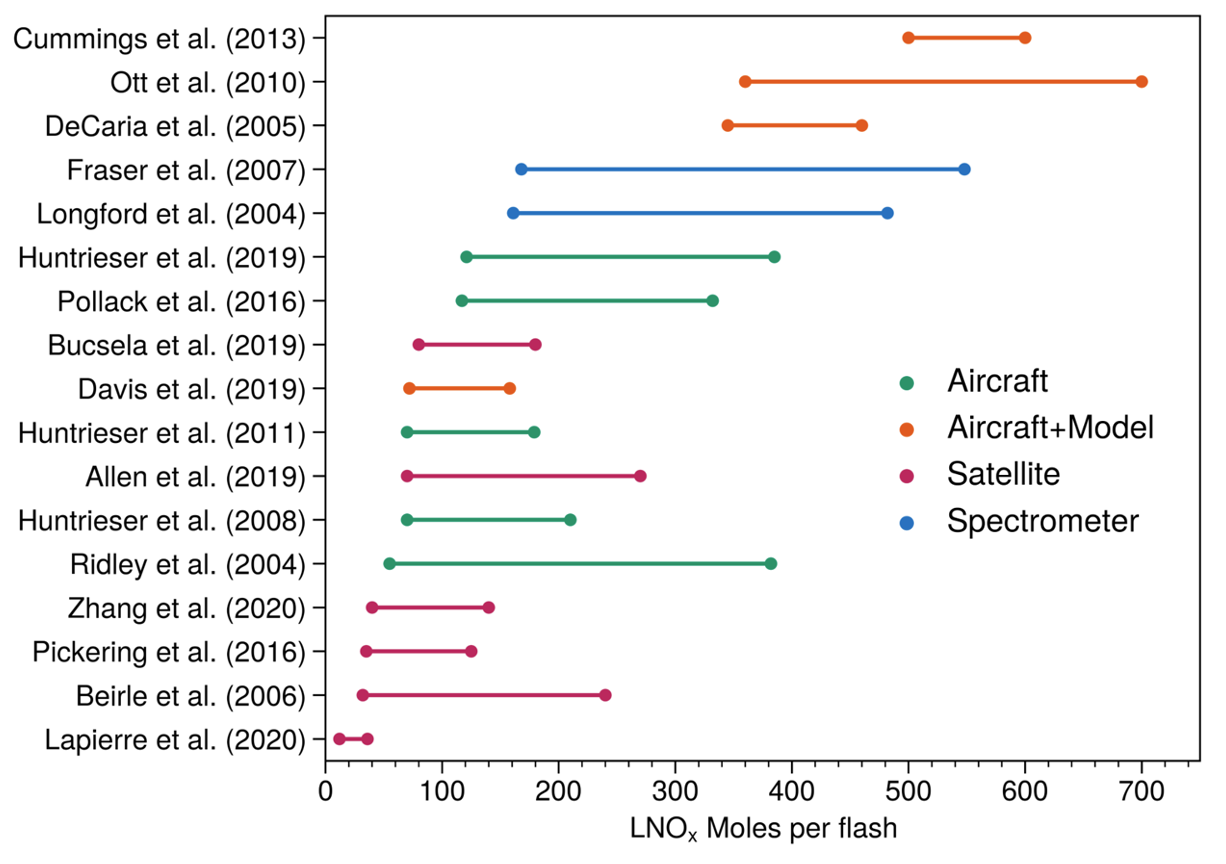
\includegraphics[width=0.9\textwidth]{./figures/lnox_production_xin.png}
\caption{近二十年不同方法所估算的LNO$_x$产率\\
Figure \ref{figure:lnox_production_xin}. Estimates of LNO$_x$ production efficiency in the recent 20 years.}
\label{figure:lnox_production_xin}
\end{figure}

尽管模式模拟和卫星观测在对流研究中很普遍,但地面差分吸收光谱仪也很有价值,并已在一些研究工作中得到应用。
由于雷暴云中云粒子的米散射和化学反应,探测到的斜柱浓度会大大增加\citep{Erle.1995,Pfeilsticker.1998,Winterrath.1999}。
因此,光学路径可由差分光学吸收光谱(DOAS)和颜色指数得出\citep{Veitel.1998,Wagner.1998},
其中颜色指数是两种不同波长下光强的比值,已被广泛用于云探测和云分类\citep{Wagner.2014,Wang.2015,Wagner.2016}。
另一方面,LNO$_x$可以使用同一仪器得出,但需要仔细地分离不同的来源。
\citet{Noxon.1976}根据以下几个假设,
1)所有观测到的NO$_2$都在云层和地面之间,
2)在分析时间内,闪电活动仍在进行,
3)NO$_2$没有明显损失,
得到LNO$_x$产率的下限为:每个CG产生约10$^{26}$个NO$_2$分子。
由于光谱仪只能检测到NO$_2$,\citet{Franzblau.1989}利用NO$_x$分析仪中NO与NO$_x$的比例,推算出每次闪电产生3$\times$10$^{27}$个NO$_x$分子。
\citet{Langford.2004}重点研究了科罗拉多雷暴个例下部产生的NO$_x$,
并使用光谱测量和NLDN数据估算出每个CG生成5.8 $\pm$ 2.9$\times$10$^{26}$个NO$_x$分子。
值得注意的是,该光谱仪于777.4 nm处记录的闪电信息与光学瞬态检测器(OTD)所用波段一样,包括IC和CG。
此外,\citet{Fraser.2007}在萨斯克彻温省使用两台DOAS仪器,
开发了两种方法(NO$_2$与O$_4$的比例和特定的大气质量因子)来得出每次CG产生6.43--7.88$\times$10$^{26}$个NO$_2$分子,
若将IC个数加入闪电个数的计算,则每次总闪产生1.01--3.30$\times$10$^{26}$个NO$_2$分子。

目前我国针对LNO$_x$的研究较少,现有的工作主要是结合理论计算,
估算局地LNO$_x$产量\citep{DuJian.2002,ZhangYiJun.2002,ZhouYunJun.2002},
得到的中国地区LNO$_x$年产量不确定范围达两个量级。
\citet{ZhouYunJun.2004}基于地闪定位网的闪电资料,通过假设单次闪电的能量,外推得到全国内陆LNO$_x$的产量为0.38 吨氮每年。
他们在估算中所用的地闪观测资料局限于广东、陇东、北京以及东北地区,存在一定的特殊性,
且在外推中选取的单次地闪能量为6.7$\times$10$^9$ J \citep{Price.1997a,Price.1997b},
该值为单次闪电产生能量的上限值 \citep{Wang.1998},因此该估算值可能偏大。
\citet{SunAnPing.2004}基于OTD的总闪观测资料,
假设单次闪电能量为4.5$\times$10$^7$ J,
没有考虑光学厚度对光能的影响及从光能到总能量的反演,
因此该值比闪电本身的能量要小,从而可能使其估算结果偏小,仅为0.016 吨氮每年。
近年来国内也有学者使用卫星观测来估算LNO$_x$,但是基于月平均或季平均数据且聚焦于清洁地区。
如通过分析青藏高原闪电活动和NO$_2$垂直柱浓度,发现LNO$_x$抑制了夏季青藏高原O$_3$低谷,且中国内陆地区LNO$_x$的年均产量为0.15(0.03--0.38)吨氮每年 \citep{JuXiaoYu.2015,Guo.2017,GuoFengXia.2019,Li.2022}。


% \subsection{深对流对痕量气体的垂直输送}
\subsection{深对流对痕量气体垂直分布的影响}

深对流云对大气化学成分的垂直输送,是近三十年来国际大气科学界一直高度关注的科学问题,
在TOGA-COARE\citep{Webster.1992}、TRACE-A\citep{Fishman.1996}和TRACE-P\citep{Jacob.2003}等一些重大国际合作项目中有关深对流的课题占了很大比重。
先后组织了一系列专门研究深对流云在大气化学成分再分布方面的大型综合观测试验,
其中包括于1998 年在欧洲进行的闪电与氮氧化物试验EULINOX\citep{Holler.2000}、
2002 年在佛罗里达进行的CRYSTAL-FACE 试验\citep{Toon.2003}、
2003至2005年在巴西实施的欧共体项目TROCCINOX\citep{Huntrieser.2008},
以及2012年在美国进行的深对流云和化学试验DC3\citep{Barth.2019}]等。
在这些试验中,深对流云对气溶胶、O$_3$前体气体以及闪电对对流层上层NO$_x$和O$_3$浓度的影响是研究的重点。
与此同时,各种尺度和复杂程度的数值模式也用于模拟和分析外场观测结果。

深对流输送边界层痕量气体至UTLS的能力,取决于各气象和化学要素。
在1985年PRESTORM的风暴尺度观测项目中,深对流输送导致对流层上层一氧化碳(CO)浓度显著增加\citep{Dickerson.1987,Pickering.1989}。
然而,在6月17日的个例中,对流层上层出流区的CO混合比与背景水平相似。这是由于冷锋过境并阻止了边界层空气直接进入云层,从而边界层上方的空气主导了入流区\citep{Pickering.1988}。
因此,天气尺度背景在深对流输送作用中起着重要作用。

除天气尺度背景外,边界层条件和动力结构也影响着深对流的输送效率。
1989年北达科他州雷暴观测项目中的中尺度对流复合体(MCC)的模拟结果表明,边界层越潮湿,对流输送能力越强,从而更多的CO被输送至云砧\citep{Stenchikov.1996}。
其他一些对流个例研究表明,深对流的输送能力与对流的垂直速度以及传输速度密切相关\citep{Pickering.1992a,Wang.1996}。
\citet{Bigelbach.2014}通过模拟2007年美国南部大平原对流季节的传输,发现准绝热强对流(QISC)比中尺度对流系统(MCS)具有更强和更深的通量,即不同类型的对流系统具有不同的输送能力。
\citet{Li.2017b}通过对比热泡对流、超级单体和MCS三种不同类型的对流系统,发现超级单体的痕量气体输送能力最强。
这是由于超级单体受质量通量的垂直梯度影响更大,而不是痕量气体混合比的垂直梯度。

入流区的结构也影响着深对流的输送能力。针对美国国家航空航天局(NASA)亚马逊边界层实验(ABLE)的观测,
\citet{Scala.1990}使用二维云模式研究了热带飑线内空气的运输途径。
气团轨迹分析表明,输送到云砧的空气中有50\%以上来自对流层中部(6 km或以上),而不是边界层。
进入对流核上升气流的空气中,50\%以上的气团被限制于5 km以下,仅约15\%的边界层空气直接传输至12 km附近的云层。
另一方面,在亚马逊干旱季节,巴西生物质燃烧区的对流个例显示,大量的O$_3$前体物被垂直输送至对流层上层,导致对流层上层O$_3$的产生大量增加\citep{Pickering.1992,Pickering.1992a,Pickering.1996}。
湿季和干季等效位温垂直廓线的巨大差异,导致对流输送特性的差异。针对中纬度地区的个例研究表明,大部分输送至UTLS的气团来源于边界层\citep{Mullendore.2005,Skamarock.2000}。

在深对流输送研究中,云参数化和云分辨模式均具有广泛应用。深对流对痕量气体的传输模拟需要真实地再现天气尺度背景、边界层结构、对流演变过程、入流区结构以及周围的化学成分。 气象研究与预报(WRF)模式是为气象研究和数值天气预报设计的三维可压非静力大气模式。
气象与化学耦合模式(WRF-Chem)是结合了大气化学的WRF模式,可以同时模拟气象学中痕量气体和气溶胶的排放、传输、混合和化学反应\citep{Fast.2006,Grell.2005}。
\citet{Barth.2012}首次在整个美国大陆上以4 km的高分辨率运行WRF-Chem模式,研究北美季风早期阶段的对流输运和化学反应。
之后,许多研究利用WRF-Chem模拟从边界层到对流云砧区的输送个例\citep{Bela.2016,Li.2017b,Li.2018}。
痕量气体的次网格对流传输是云参数化模拟的重要组成部分。
\citet{Wang.1996}针对TRACE-A观测的热带MCS和PRESTORM观测期间的飑线,利用多层嵌套探讨了次网格尺度和网格尺度对流传输的差异。
其中MCS个例使用90和30 km两层嵌套,飑线个例使用75和25 km两层嵌套。
研究发现,在上升气流中发生了大量的次网格传输(在MCS个例中约占总向上传输的41\%,在飑线个例中约占64\%)。
\citet{Ott.2009}将云分辨模式(CRM)和柱模式(SCM)对三种对流系统中痕量气体垂直分布的模拟结果进行了比较。
他们发现,相对于CRM,SCM低估了对流层上部的对流质量通量和痕量气体混合比。
此外,他们也研究了SCM中对流传输对微物理方案参数值的敏感性。
通过调整影响对流传输的最重要参数,改进了SCM对痕量气体混合比的模拟。
\citet{Freitas.2000}针对低分辨率大气模式,提出了与深对流系统相关的次网格痕量气体对流输送的参数化。
\citet{Grell.2014}详细描述了次网格对流参数化、示踪气体传输和湿清除计算方法,该方法可用于高分辨率非静力中尺度模式。
\citet{Li.2018}通过对比不同的对流参数化(12和36 km)和云分辨模拟结果,
指出对流参数化模拟的对流输送比云分辨模拟结果要弱,并且该输送能力在对流早期而不是后期受对流参数化的控制更多。
因此,对流输送参数化与次网格对流云方案需一致,且对流参数化需要能够真实反映冰相的微物理。

在对流层上层中形成的O$_3$和气溶胶的多少,取决于净对流输送的液相和/或冰相中可溶并具有反应性的气体。
在对流层上层中,O$_3$的形成需要NO$_x$和HO$_x$,其机理为HO$_2$和有机过氧自由基(RO$_2$)将NO氧化,
然后NO$_2$光解,激发态O原子与O$_2$分子结合。
但是,由于HO$_x$的寿命短,因此对流层上层中HO$_x$的量取决于寿命更长的HO$_x$前体物的含量\citep{Chatfield.1984,Prather.1997},
例如过氧化氢(H$_2$O$_2$),甲基过氧化氢(CH$_3$OOH)和甲醛(CH$_2$O),
这些前体物是可溶的,且具有液相的化学源和汇\citep{Barth.2007,Carlton.2007}。
H$_2$O$_2$是由HO$_2$自由基与其自身反应形成的。 CH$_2$O和CH$_3$OOH来自于CH$_4$和其他碳氢化合物的氧化。
对流层上层的NO$_x$除了来源于LNO$_x$,也受对流输送的边界层NO$_x$以及硝酸(HNO$_3$)影响\citep{Grassian.2005},
而HNO$_3$很容易被云水和冰粒清除\citep{Neu.2012}。
通过比较DC3项目中入流区和出流区内的痕量气体,可知CH$_3$OOH的清除效率(12--84\%)很大程度上取决于冰相保留系数,
但H$_2$O$_2$(80--90\%)和CH$_2$O(40--60\%)并非如此\citep{Barth.2016,Bela.2016,Fried.2016}。
\citet{Cuchiara.2020}指出,与SEAC4RS观测中CH$_3$OOH清除率(4\%--27\%)相比,DC3观测中其清除率更高,该现象很大程度上可由冰相保留系数解释。
有关DC3项目的研究总结(如垂直输送、湿清除、LNO$_x$及平流层-对流层交换等)详见\citet{Barth.2019}。

我国的研究人员在深对流云对污染物的垂直输送方面也做了有意义的探索。
\citet{GaoHuiWang.1998}利用一个欧拉型硫沉降模式,研究了积云对硫污染物垂直输送的作用。
他们的结果表明,积云引起的垂直气流可使对流层高层的硫污染物浓度增加50--400\%。
\citet{LiBing.1999,LiBing.2001}则利用一个耦合的冰雹云-化学模式模拟了
我国陕西一次单体积云对流的发展过程及其对对流层O$_3$和NO$_x$等化学成分再分布的作用。他们的模拟结果表明,
云内强烈的垂直输送能在30分钟左右把低层低体积分数的O$_3$和高体积分数的NO$_2$快速、
有效地输送到对流层的上部,造成化学物种的再分布。
\citet{HuJiaYing.2019}利用带有详细分档微物理方案及液相化学的云模式,
对2014年7月30日发生在安徽滁州境内一次深对流过程进行了模拟研究。
研究结果表明,在积云发展阶段,强上升气流使得云内源层示踪气体有效地向上输送,
对流层中部强的夹卷过程及水平入流使得云外气体入云输送至主要对流区,并在垂直气流的作用下进一步影响各层示踪气体的分布。
各层示踪气体均可向上输送至对流层上部,其中对流层中部示踪气体(2.1--4.5 km、4.5--7.5 km 和 7.5--10.8 km)的向上输送作用与近地层示踪气体(0--2.1 km)的贡献相当。

% \subsection{闪电氮氧化物的影响}



\section{存在问题及本研究目标和研究内容}

总体而言,我国在大气污染物垂直输送及相关物理化学过程和机制方面的研究还很少,即使有,也比较零散,
特别是缺少对对流输送相关事实的观测认知,这与近几年开展较多的地面大气污染观测和模拟研究不相称。
所以,进行对大气污染物垂直输送过程、机理及其影响的研究,对全面理解和预测其环境、气候效应都具有不可替代的作用。
而探索闪电对对流层上层NO$_x$和O$_3$产量的贡献,是理解深对流云对大气成分垂直分布影响的另一个重要方面。

具体而言,有以下科学问题亟待研究:

\begin{enumerate}[label=(\arabic*), labelindent=\parindent, leftmargin=0pt, widest=0, itemindent=*, topsep=0pt, partopsep=0pt, parsep=0pt]

\item 由于原位观测有限,如何利用卫星资料得到不同污染程度地区的LNO$_2$柱浓度和产率?

\item LNO$_2$的产率与哪些因素有关?对闪电NO$_x$的产量有何影响?

\item 除了LNO$_2$柱浓度,能否利用卫星资料得到对流云的NO$_2$和O$_3$廓线并进行来源分析?

\item 针对不同的深对流系统,动力输送和化学反应如何影响O$_3$的垂直再分布?其中LNO$_x$又起到了什么作用?

\end{enumerate}

\begin{figure}[H]
\centering
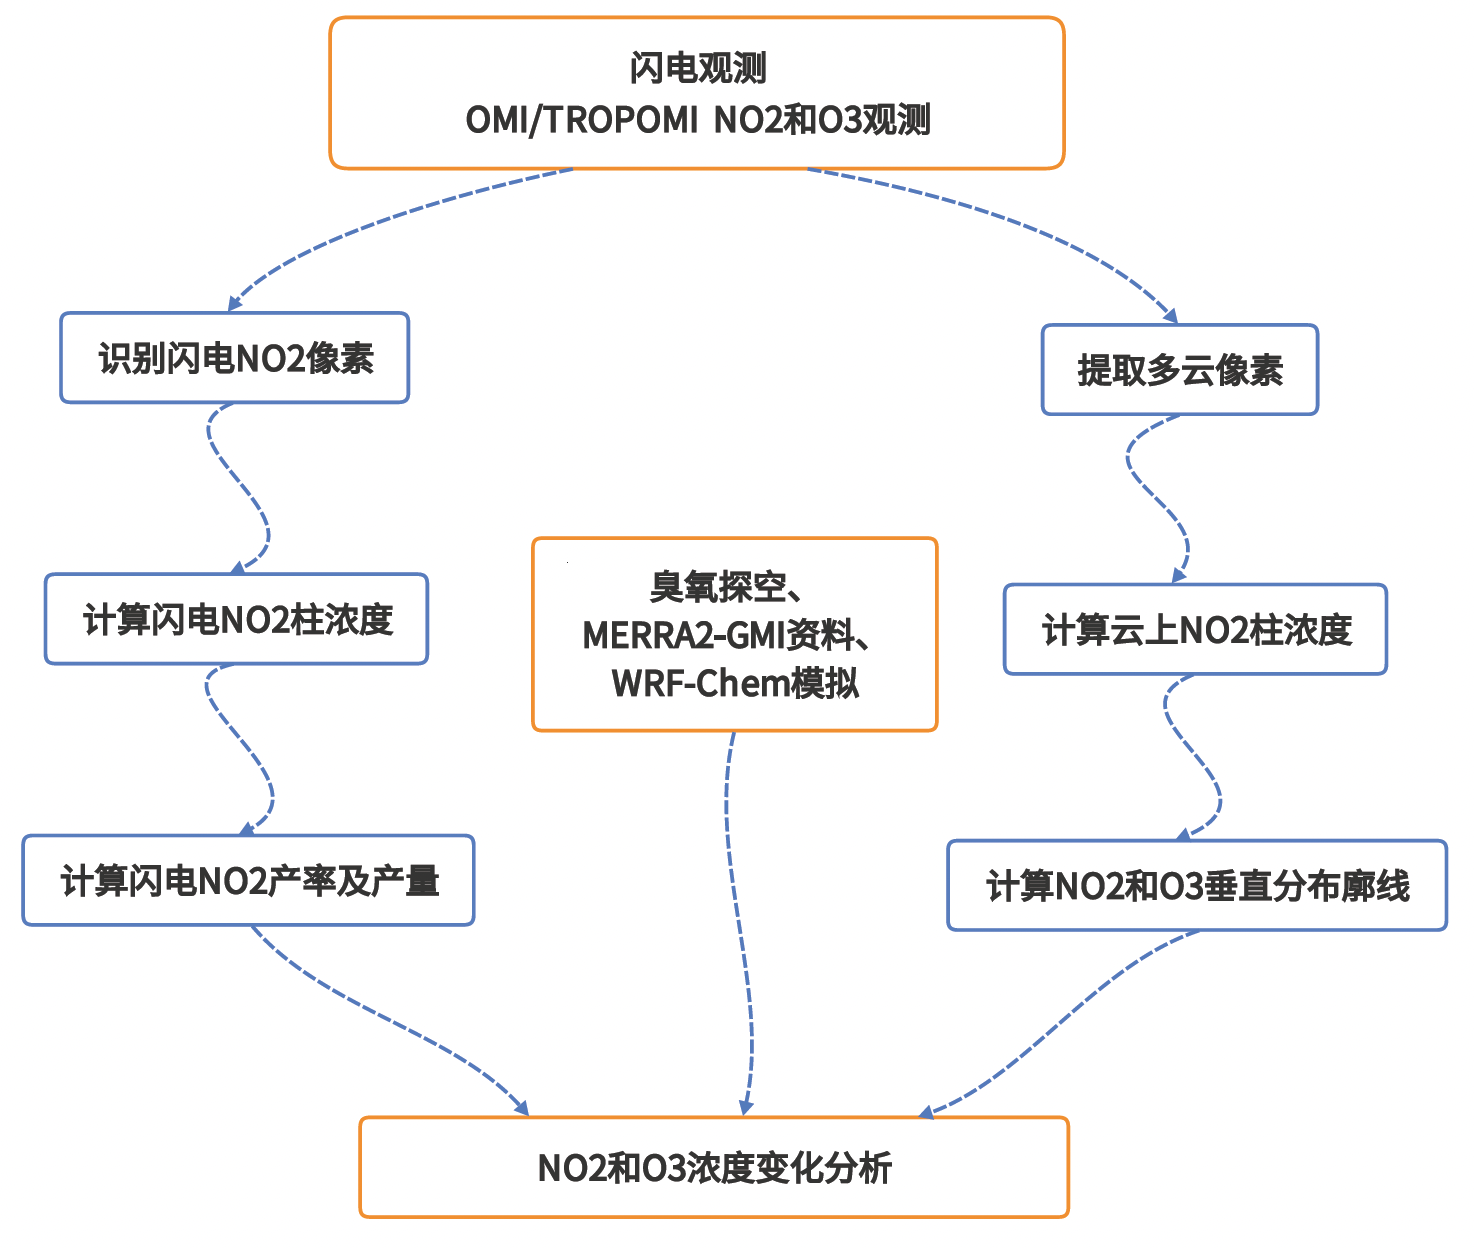
\includegraphics[width=0.9\textwidth]{./figures/schematic_diagram.png}
\caption{技术路线图。\\
Figure \ref{figure:schematic_diagram}. Schematic diagram.
}
\label{figure:schematic_diagram}
\end{figure}

针对以上问题,本文的研究目标为:

\begin{enumerate}[label=(\arabic*), labelindent=\parindent, leftmargin=0pt, widest=0, itemindent=*, topsep=0pt, partopsep=0pt, parsep=0pt]

\item 利用更准确的NO$_2$先验廓线,开发适用于清洁和污染地区的LNO$_2$柱浓度产品,进而估算LNO$_2$的产率。

\item 将卫星得到的多种二级产品与闪电数据相结合,分析闪电NO$_x$的产率与云属性和闪电属性的关系。

\item 将前人的云切片算法用于不同高度的对流云,探讨其适用条件和得到的NO$_2$和O$_3$廓线分布,并与模拟结果进行对比分析,从而确认差异来源。

\item 针对中国地区不同的深对流系统开展联合观测,为模式模拟提供可靠数据(雷达产品、闪电定位信息以及O$_3$廓线),
并利用评估后的模式结果来进一步研究动力输送、化学反应和LNO$_x$的作用。

\end{enumerate}


技术路线见图\ref{figure:schematic_diagram}。

本文研究内容与章节安排如下:

第一章:阐述本文的选题依据和意义,从原位观测、模式模拟以及卫星观测的角度回顾了
1)深对流云对大气化学成分的垂直输送,
2)闪电NO$_x$的产率估算及其对其他痕量气体的影响,
提出本文的科学问题和研究内容。

第二章:介绍本文的资料来源和研究方法,对论文中使用的模式和反演方法进行简要介绍。

第三章:开发适用于不同地区的LNO$_2$算法,分析北极、美国大陆以及中国东南部的LNO$_2$产率,并与其他NO$_x$排放源进行对比。
分析LNO$_2$产率与海陆差异和闪电频率之间的关系,并量化其对LNO$_2$产量的影响。

第四章:将云切片算法得到的NO$_2$廓线与相同条件下模式模拟的NO$_2$廓线进行对比分析,并利用模式的敏感性试验探讨LNO$_2$对NO$_2$柱浓度的重要性。

第五章:利用已得的NO$_2$廓线和模式结果,分析云切片算法得到的不同地区O$_3$垂直分布。
此外对中国东南部的联合观测试验进行分析,并利用模式具体分析不同类型的深对流系统对O$_3$的影响,
得到动力输送、化学反应及LNO$_x$在其中所起的作用。

第六章:对全文进行总结,提炼结论,并讨论论文的创新点并探讨研究的不足之处以及对于未来工作的展望。
